\documentclass[journal]{IEEEtran}
\usepackage{amsmath,amsfonts}
\usepackage{algorithmic}
\usepackage{algorithm}
\usepackage{array}
\usepackage[caption=false,font=normalsize,labelfont=sf,textfont=sf]{subfig}
\usepackage{textcomp}
\usepackage{stfloats}
\usepackage{url}
\usepackage{verbatim}
\usepackage{graphicx}
\usepackage{booktabs}
\usepackage{cite}
\usepackage{etoolbox}
\usepackage{placeins}
\makeatletter
% Tighter title/author/header block without changing type sizes (\Huge title, \sublargesize author, header font).
\def\IEEEtitletopspace{0.28\baselineskip}
\def\IEEEtitletopspaceextra{-2.5pt}
\def\@IEEENORMtitlevspace{1.85\baselineskip}
\def\@IEEEMINtitlevspace{1.45\baselineskip}
\addtolength{\headsep}{-5pt}
\patchcmd{\@maketitle}{\vskip0.2em}{\vskip0.06em}{}{}
\patchcmd{\@maketitle}{\vskip1.0em\par}{\vskip0.58em\par}{}{}
\patchcmd{\@maketitle}{\lineskip.5em\@IEEEcompsoconly{\sffamily}\sublargesize}{\lineskip.35em\@IEEEcompsoconly{\sffamily}\sublargesize}{}{}
\patchcmd{\@maketitle}{\addvspace{0.5\baselineskip}}{\addvspace{0.3\baselineskip}}{}{}
\makeatother
\renewcommand\thesection{\arabic{section}}
\renewcommand\thesubsection{\thesection.\arabic{subsection}}
\renewcommand\thesectiondis{\thesection.}
\renewcommand\thesubsectiondis{\thesectiondis\arabic{subsection}.}
\hyphenation{op-tical net-works semi-conduc-tor IEEE-Xplore
  do-main-spe-cific param-eter-ef-fi-cient resource-in-ten-sive
  do-main-adap-ted vis-ion-lan-guage under-water}
\setlength{\emergencystretch}{1.25em}
\setlength{\floatsep}{6pt plus 2pt minus 2pt}
\setlength{\textfloatsep}{8pt plus 2pt minus 4pt}
\setlength{\intextsep}{6pt plus 2pt minus 2pt}
\setlength{\abovecaptionskip}{4pt}
\setlength{\belowcaptionskip}{0pt}
\tolerance=2500
\pretolerance=200
\hbadness=5500

\begin{document}

\title{Domain Specialized BLIP-2 for Underwater Image Captioning:\\A Lightweight Approach for Marine Robotics}

\author{James Nguyen, 301582186\\ Kevin Tang, 301357455\\ Mason Liang, 301361725}

\markboth{CMPT 420 Project Report}{BLIP-2 Explorer: Underwater Image Captioning}

\maketitle

\begin{abstract}
Marine robotics and ecological monitoring produce large volumes of underwater imagery, yet turning this footage into searchable text requires vision language models that are both domain aware and deployable on embedded hardware. Existing models are either too large for on device use or too generic to handle underwater visual challenges such as color attenuation, low contrast, and domain specific subjects. We introduce \textbf{BLIP-2 Explorer}, a lightweight captioning pipeline that adapts BLIP-2 to underwater imagery via low rank adaptation (LoRA) and compresses it further through knowledge distillation into a compact BLIP-1 student. Training uses a composite objective combining cross entropy loss with a CLIP auxiliary alignment term; checkpoint selection uses a weighted composite of five caption metrics to prevent metric gaming.
\end{abstract}

\section{Introduction \& Motivation}

\IEEEPARstart{U}{nderwater} and marine environments are increasingly monitored by AUVs, ROVs, and fixed seafloor sensors, generating continuous image and video streams for ecological surveys, infrastructure inspection, and search and recovery operations. Translating this visual data into natural language descriptions would enable full text search over footage archives, semi automated annotation, and post mission summaries, without requiring an operator to manually review hours of video.

Image to text captioning is the natural solution, yet several constraints make deployment difficult. Marine platforms operate with poor or absent connectivity, so inference must be on device. Available compute and memory budgets are far smaller than those assumed by state of the art captioning systems. Underwater imagery is also visually distinct from natural image pretraining data: water absorbs red wavelengths, producing a pervasive blue green color cast; backscatter from suspended particles lowers contrast; turbidity varies dramatically with depth and water conditions; and objects of interest (fish, coral, seafloor structure, marine debris) are severely underrepresented in generic pretraining corpora. General purpose models face two challenges simultaneously: being too large and too poorly calibrated for this domain.

Despite these degradations, large image encoders learn shape and texture features that are more robust to color shift than to structural change. A blue green color cast biases the histogram but preserves object contours and textural cues. The core challenge is not recognizing that fish or coral are present, but producing precise captions that name species, describe behaviors, and use the vocabulary marine biologists write. This vocabulary gap, rather than low level perception failure, is the bottleneck that LoRA adaptation targets.

We start from BLIP-2~\cite{ref3}, whose modular design exposes a small, learnable Q-Former bridge between a frozen image encoder and a frozen language model, making it a practical target for parameter efficient adaptation. We apply LoRA~\cite{ref1} to inject rank decomposed perturbations into the Q-Former and decoder with minimal compute overhead. To compress the result for embedded deployment, we apply knowledge distillation~\cite{ref2}, training a compact BLIP-1 student to mimic the LoRA adapted BLIP-2 teacher.

The main contributions are: (1) a LoRA adaptation recipe for BLIP-2 on underwater imagery with standardized multi metric evaluation; (2) a composite training objective and checkpoint selection metric that prevent single metric gaming; (3) a quantitative analysis of the domain gap and how LoRA closes it; (4) identification and remediation of a degenerate period suffix output artifact that collapses ngram metrics; and (5) a distilled BLIP-1 student trained with knowledge distillation that achieves a $4\times$ memory reduction with competitive captioning quality.

\section{Related Work}

\subsection{BLIP-2 and Vision Language Pretraining}
BLIP-2~\cite{ref3} connects two frozen unimodal models, a large image encoder and a large language model, via a lightweight Querying Transformer (Q-Former). The Q-Former holds 32 learnable query tokens that cross attend to frozen image features, compressing visual information into a compact representation. Stage~1 pretraining aligns vision and language via contrastive learning and image grounded text generation; Stage~2 projects Q-Former outputs into the LLM embedding space as soft visual prompts. Because only the Q-Former and projection layer are trained, approximately 188M of 3.4B parameters require adaptation. Recent work on efficient Q-Former alignment~\cite{ref6} confirms that targeted Q-Former adaptation yields competitive results, supporting our choice to focus LoRA on this module.

\subsection{Parameter Efficient Fine Tuning and LoRA}
LoRA~\cite{ref1} freezes pretrained weights $W_0$ and learns a low rank update $\Delta W = BA$, where $B \in \mathbb{R}^{d \times r}$, $A \in \mathbb{R}^{r \times k}$, $r \ll \min(d,k)$. During training only $A$ and $B$ are updated; at deployment they are merged into $W_0$ with no added latency. LoRA reduces trainable parameters to a fraction of the full model (as low as 0.01\% for GPT-3 175B~\cite{ref1}), making fine tuning practical on constrained hardware.

\subsection{Knowledge Distillation}
Knowledge distillation~\cite{ref2} trains a smaller student to mimic a larger teacher's output distributions, reducing size and latency while retaining domain specific behavior. In our pipeline, the LoRA augmented BLIP-2 OPT-2.7B serves as the teacher and a LoRA adapted BLIP-1 serves as the compact student. Rather than training on the original UICD ground truth captions, the student is trained on pseudo labels: captions generated by the frozen teacher over the training split. The same composite loss (Eq.~\ref{eq:loss}) and hyperparameters are used. Both models are then evaluated on the same held out test set with the original ground truth references, so test metrics are directly comparable. One caveat is that the student's validation loss during training reflects divergence from teacher pseudo labels rather than ground truth, introducing some uncertainty when interpreting epoch level training curves; however, the final test scores reported in Table~\ref{tab:results} are computed against the same references for all models.

\subsection{Domain Specific Captioning}
MedBLIP~\cite{ref4} adapts BLIP to 3D medical imagery, showing that the architecture transfers to niche visual domains with domain aligned supervision. PixLore~\cite{ref5} shows that enriching training captions with detailed descriptors improves domain vocabulary coverage. Underwater imagery is comparably challenging: uncontrolled lighting, turbidity, and color distortion vary with depth and water clarity, and UICD, one of few public marine captioning datasets, contains only 3,176 images.

\FloatBarrier
\section{Method}
\subsection{Dataset and Preprocessing}
We use UICD: 3,176 JPEG images at 224$\times$224 pixels of marine scenes (fish, turtles, coral, seafloor), each with five human written reference captions. A deterministic 80/10/10 split (seed 42) yields 2,540 training, 317 validation, and 319 test images. The images span the full range of underwater degradations: color casts from light cyan (shallow) to deep blue green (depth), motion blur from swimming subjects, turbidity haze, and strong brightness variation. During training, one of the five reference captions is sampled randomly per image per step, exposing the decoder to diverse sentence structures and synonym choices without requiring additional images. We do not apply explicit color correction; LoRA instead learns implicit compensations for domain specific color statistics directly from the training distribution, avoiding enhancement artifacts.

\subsection{Baseline and Metrics}
The baseline is frozen BLIP-2 OPT-2.7B evaluated on the test set. Evaluating with a single metric is risky: optimizing CLIP alone can yield generic captions (e.g., ``an underwater image'') that score well despite being uninformative. We therefore report CLIP similarity (OpenCLIP ViT-B-32), CIDEr, SPICE, METEOR, BLEU-4, and ROUGE-L.

Checkpoint selection uses a composite validation score:
\begin{equation}
  S = \sum_{m} w_m \cdot s_m / c_m,
  \label{eq:composite}
\end{equation}
with weights: CLIP (0.50), CIDEr (0.25), METEOR (0.10), BLEU-4 (0.08), ROUGE-L (0.07); normalization $c_m = 2.0$ for CIDEr and 1.0 otherwise. Fig.~\ref{fig:composite_both} shows the composite score for both models over training, with the best checkpoint selected at epoch~1 in each case.

\begin{figure}[htbp]
  \centering
  \subfloat[LoRA teacher. Best checkpoint at epoch~1 (red dot).\label{fig:composite}]{%
    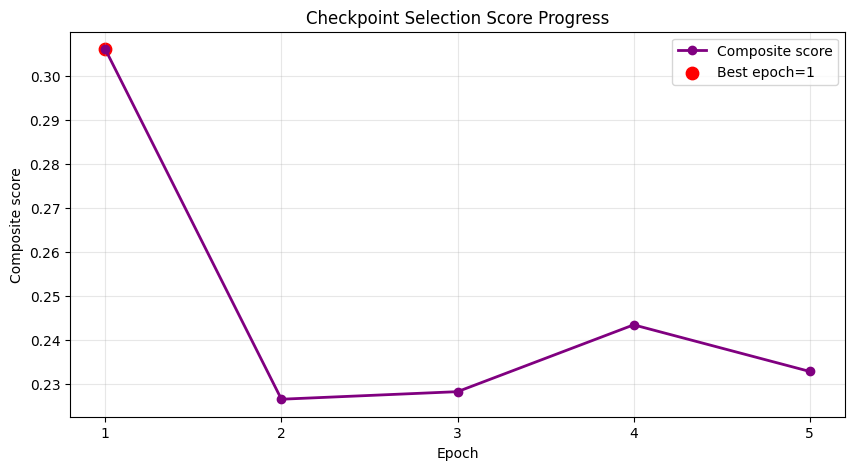
\includegraphics[width=0.9\columnwidth]{graphs/composite_score_curve.png}}\\
  \subfloat[Distilled BLIP-1 student. Best checkpoint at epoch~1; score oscillates thereafter.\label{fig:composite_distill}]{%
    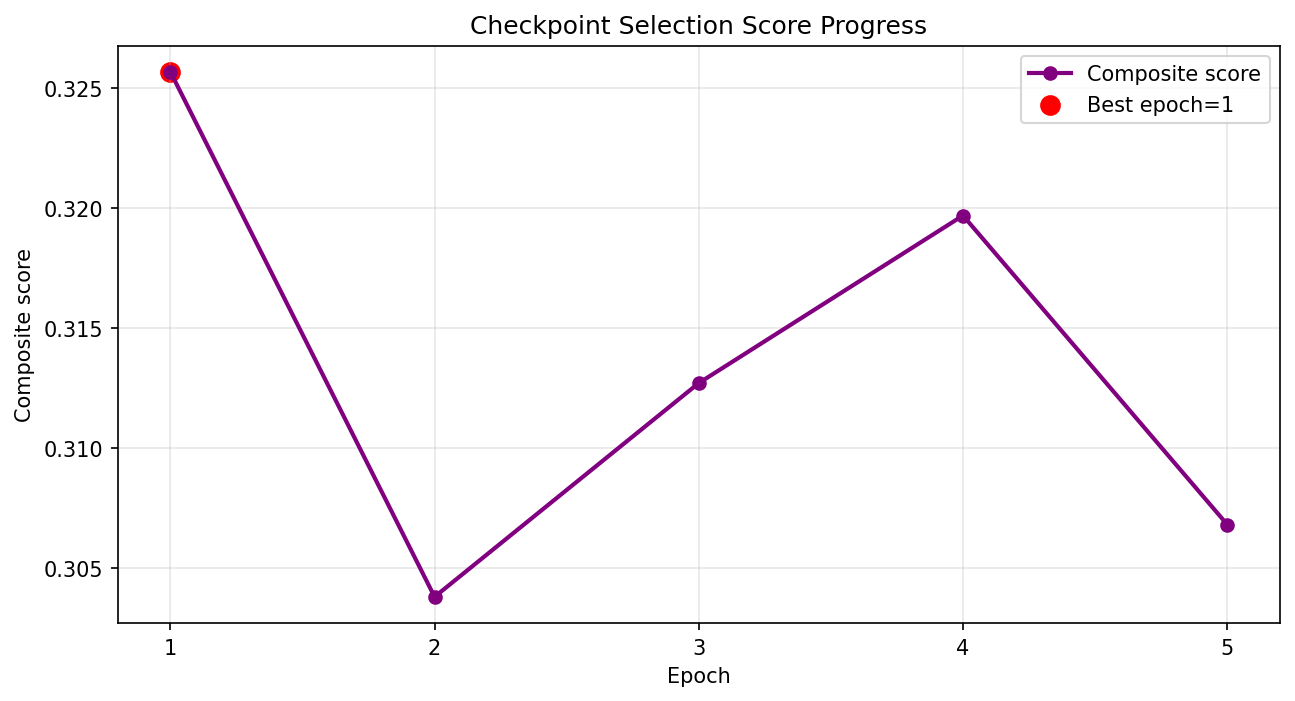
\includegraphics[width=0.9\columnwidth]{graphs/composite_score_curve_distill.png}}
  \caption{Composite checkpoint selection score (Eq.~\ref{eq:composite}) over 5 epochs for the LoRA teacher (top) and distilled student (bottom).}
  \label{fig:composite_both}
\end{figure}

\subsection{Training Objective}
The training loss combines language modeling cross entropy with a CLIP auxiliary alignment term:
\begin{equation}
  \mathcal{L} = \mathcal{L}_{\mathrm{CE}} + \alpha \cdot \mathcal{L}_{\mathrm{CLIP\_aux}},
  \label{eq:loss}
\end{equation}
where $\alpha = 0.2$. The auxiliary term encourages Q-Former hidden states (projected into CLIP's embedding space) to align with the CLIP image embedding, applied every 5 steps and linearly warmed up over the first epoch.

The CLIP auxiliary loss plays a stabilizing role for the underwater domain. Without it, optimizing only cross entropy could cause the Q-Former to overfit to UICD's narrow vocabulary, producing fluent but visually ungrounded captions. The auxiliary loss anchors Q-Former representations to CLIP's joint embedding space, which encodes coarse but reliable image level semantics even for degraded underwater inputs, allowing the model to improve lexical precision through CE while remaining semantically grounded.
Both terms in Eq.~\ref{eq:loss} backpropagate into the Q-Former and decoder attention projections that the next subsection adapts with LoRA, so the composite objective supervises the same low rank pathways that carry visual grounding into token predictions.

\subsection{LoRA Adaptation}
LoRA injects trainable low rank matrices into linear projections while keeping the original weights fixed: each adapted layer implements $W + BA$ with $B \in \mathbb{R}^{d \times r}$, $A \in \mathbb{R}^{r \times k}$, and typically $r \ll \min(d,k)$, so the number of trainable parameters is orders of magnitude smaller than full finetuning of $W$.
We attach these updates to the query, key, and value projections in every Q-Former cross attention layer and in the OPT decoder self attention because those maps control how image tokens attend to text queries and how caption tokens condition on prior context; adapting them shifts the model toward marine vocabulary and scene structure without retuning the frozen ViT or the bulk of the language model.
At inference, $A$ and $B$ can be merged into the frozen weights, so deployed latency matches a single forward pass through the original linear layers.
LoRA is applied to the \texttt{q\_proj}, \texttt{k\_proj}, and \texttt{v\_proj} matrices in both Q-Former cross attention blocks and the OPT decoder, with rank $r=16$, $\alpha=16$, and dropout 0.1. All base parameters remain frozen. Training uses AdamW (lr $2\times10^{-4}$), linear warmup over 10\% of steps, batch size 3, for 5 epochs across two T4 GPUs. The same LoRA configuration is applied to the BLIP-1 student during distillation training.

\subsection{Output Post Processing}
The raw LoRA model generates captions with degenerate trailing period sequences: after a plausible initial phrase, the model repeatedly emits a period token (e.g., ``A group of small fish swim around the coral . . . . . . .''\!). This is a known failure mode when fine tuning autoregressive models on short, structured text. The artifact affects metrics asymmetrically: CLIP similarity is nearly unaffected, but CIDEr collapses from 1.159 (fixed) to 0.017 (raw) because repeated periods yield no informative ngram overlap with any reference.

We address this with a single regular expression that strips trailing spaced periods, restoring the caption to its meaningful prefix. The fix requires no retraining, adds negligible overhead, and is applied uniformly to all four models.

\FloatBarrier
\section{Experiments \& Results}

\subsection{Experimental Setup}
All experiments run on Kaggle Notebooks with two NVIDIA T4 GPUs (15\,GB VRAM each), loaded in fp16 with Accelerate's automatic device map partitioning layers across both GPUs. Training uses AdamW (lr $2\times10^{-4}$, weight decay 0.01), linear warmup over 10\% of steps, batch size 3 with gradient accumulation over 4 steps (effective batch size 12), for 5 epochs with gradient checkpointing enabled. For the teacher, only LoRA parameters are updated; the distilled BLIP-1 student uses the same config but trains against teacher generated pseudo labels.

Inference uses 8-bit quantization (BitsAndBytes) with beam search (3 beams, max 50 tokens, no repeat ngram size 3). Metrics are computed via \texttt{pycocoevalcap} against all five ground truth references per image; CLIP similarity uses \texttt{open\_clip\_torch} ViT-B-32 (LAION-2B). Fig.~\ref{fig:efficiency_both} compares per epoch wall clock time and peak GPU memory for both models.

\begin{figure}[htbp]
  \centering
  \subfloat[LoRA teacher: 750 to 1200\,s/epoch, $\sim$5.5\,GB GPU memory.\label{fig:efficiency}]{%
    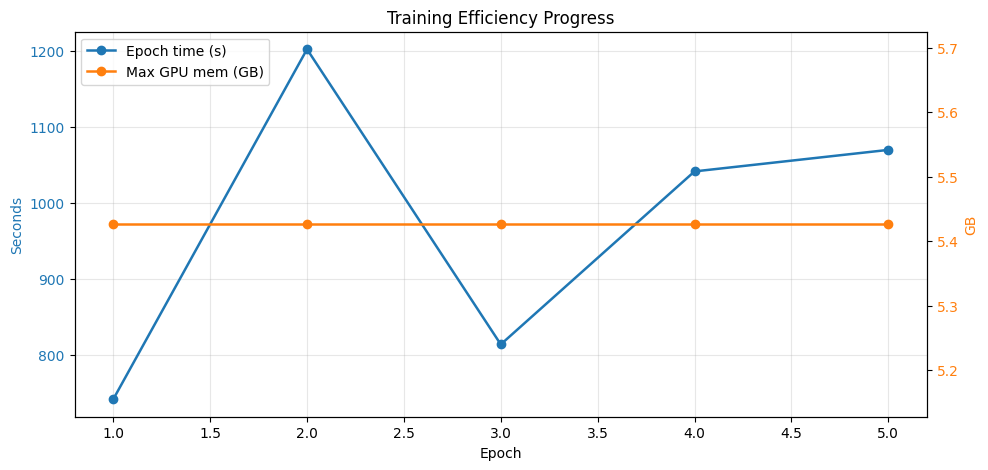
\includegraphics[width=0.9\columnwidth]{graphs/efficiency_curve.png}}\\
  \subfloat[Distilled student: 1255 to 1320\,s/epoch, $\sim$1.47\,GB GPU memory ($4\times$ reduction).\label{fig:efficiency_distill}]{%
    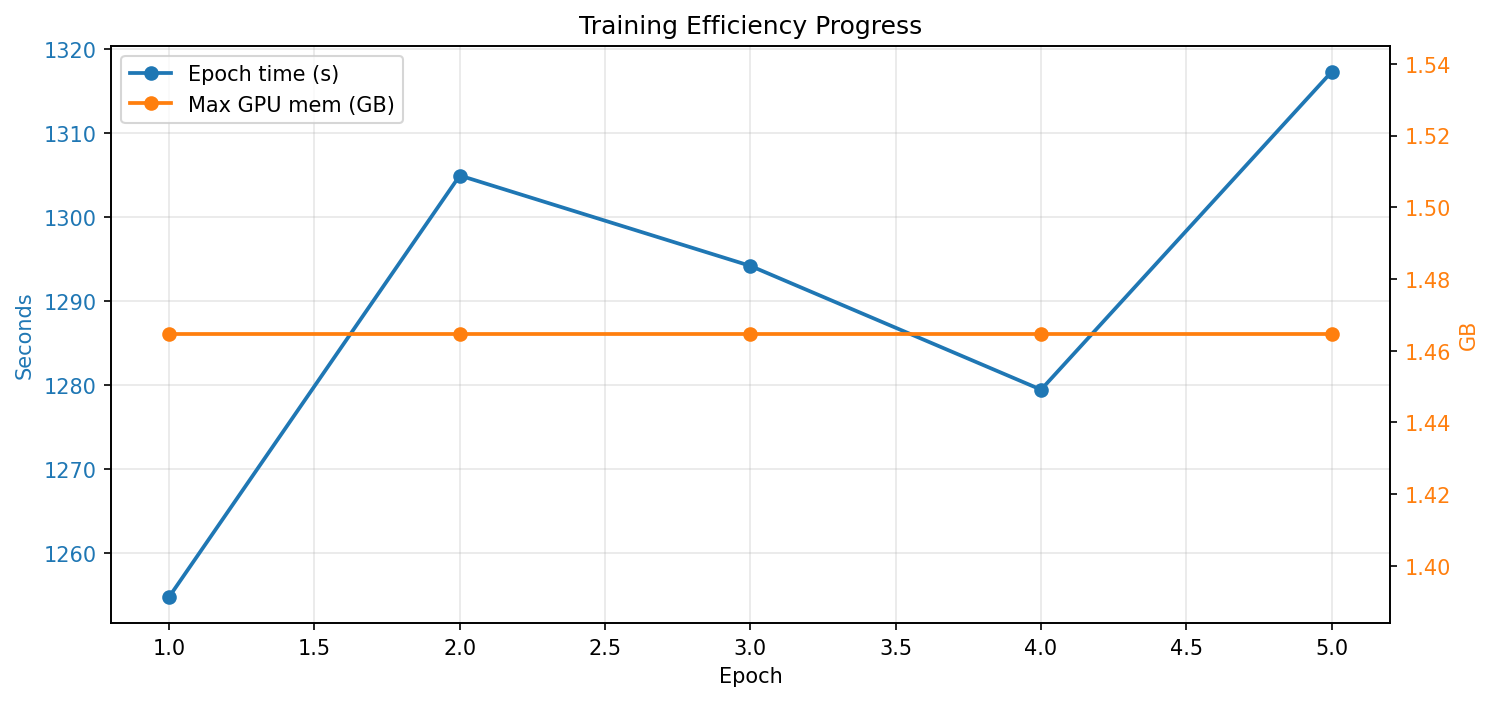
\includegraphics[width=0.9\columnwidth]{graphs/efficiency_curve_distill.png}}
  \caption{Training efficiency per epoch: wall clock time (left axis) and peak GPU memory (right axis).}
  \label{fig:efficiency_both}
\end{figure}

\FloatBarrier
\subsection{Results}

\begin{table*}[!t]
\caption{Caption quality on UICD test set (319 images). MTR = METEOR, RGE = ROUGE-L, B-4 = BLEU-4.}
\label{tab:results}
\centering
\small
\setlength{\tabcolsep}{6pt}
\begin{tabular}{@{}l r r r r r r@{}}
\toprule
\textbf{Model} & \textbf{CLIP} $\uparrow$ & \textbf{CIDEr} $\uparrow$ & \textbf{SPICE} $\uparrow$ & \textbf{MTR} $\uparrow$ & \textbf{RGE} $\uparrow$ & \textbf{B-4} $\uparrow$ \\
\midrule
Base BLIP-2          & 0.311 & 0.474 & 0.138 & 0.181 & 0.331 & 0.110 \\
LoRA BLIP-2          & 0.310 & 1.159 & 0.243 & 0.307 & 0.632 & 0.403 \\
LoRA aug.\ BLIP-2 (teacher) & \textbf{0.313} & \textbf{1.317} & \textbf{0.267} & \textbf{0.333} & \textbf{0.663} & \textbf{0.439} \\
Distilled BLIP-1     & 0.321 & 0.703 & 0.190 & 0.305 & 0.435 & 0.238 \\
\bottomrule
\end{tabular}
\end{table*}

Table~\ref{tab:results} reports test set caption quality across all four models. The base BLIP-2 model (row~1) shows a clear domain gap: CIDEr 0.47 indicates little overlap with reference vocabulary, and SPICE 0.14 suggests poor coverage of marine objects and relations. After LoRA fine tuning and post processing (row~2), all metrics improve substantially. LoRA augmented BLIP-2 (row~3) achieves the best captioning scores: CIDEr 1.32 ($+179\%$ over base), SPICE 0.27 ($+93\%$), METEOR 0.33 ($+84\%$), BLEU-4 0.44 ($+300\%$). CLIP similarity changes only marginally (0.311 to 0.313), confirming that coarse visual semantic alignment was already adequate; LoRA's main benefit is domain specific lexical and semantic precision.

The distilled BLIP-1 student (row~4) was trained on teacher generated pseudo labels and evaluated on the same test set as the other models. It trades some captioning quality for lower resource usage, achieving CIDEr 0.70 ($+48\%$ over base), METEOR 0.31 ($+71\%$), and ROUGE-L 0.44 ($+32\%$). Most metrics are retained relative to the teacher, with CIDEr showing the largest drop, consistent with it being the metric most sensitive to exact lexical overlap. Because the student trained on pseudo labels rather than ground truth, a portion of the gap may reflect label distribution differences rather than model capacity alone.

To contextualize these values: the base BLIP-2 produces generic captions such as ``a fish in the water,'' sharing few ngram overlaps with references that name species, color, and behavior. LoRA augmented BLIP-2 produces specific captions such as ``a group of yellow and black fish swimming near a coral reef,'' closely matching human written references. The distilled student produces captions of intermediate specificity, correctly identifying the scene and dominant subject but occasionally missing fine grained species detail. The $+93\%$ SPICE gain from base to LoRA augmented BLIP-2 indicates the model has learned structured scene decomposition rather than surface phrase memorization.

\begin{figure}[htbp]
  \centering
  \subfloat[LoRA teacher. CIDEr peaks at epoch~4 then declines.\label{fig:metrics}]{%
    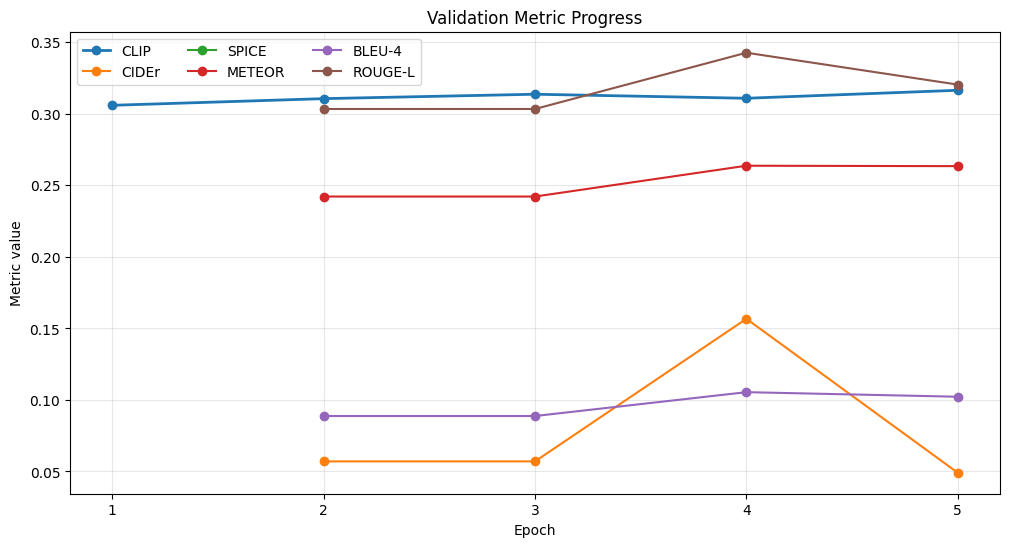
\includegraphics[width=0.9\columnwidth]{graphs/metric_curves.png}}\\
  \subfloat[Distilled student. CIDEr peaks at epoch~1 then oscillates.\label{fig:metrics_distill}]{%
    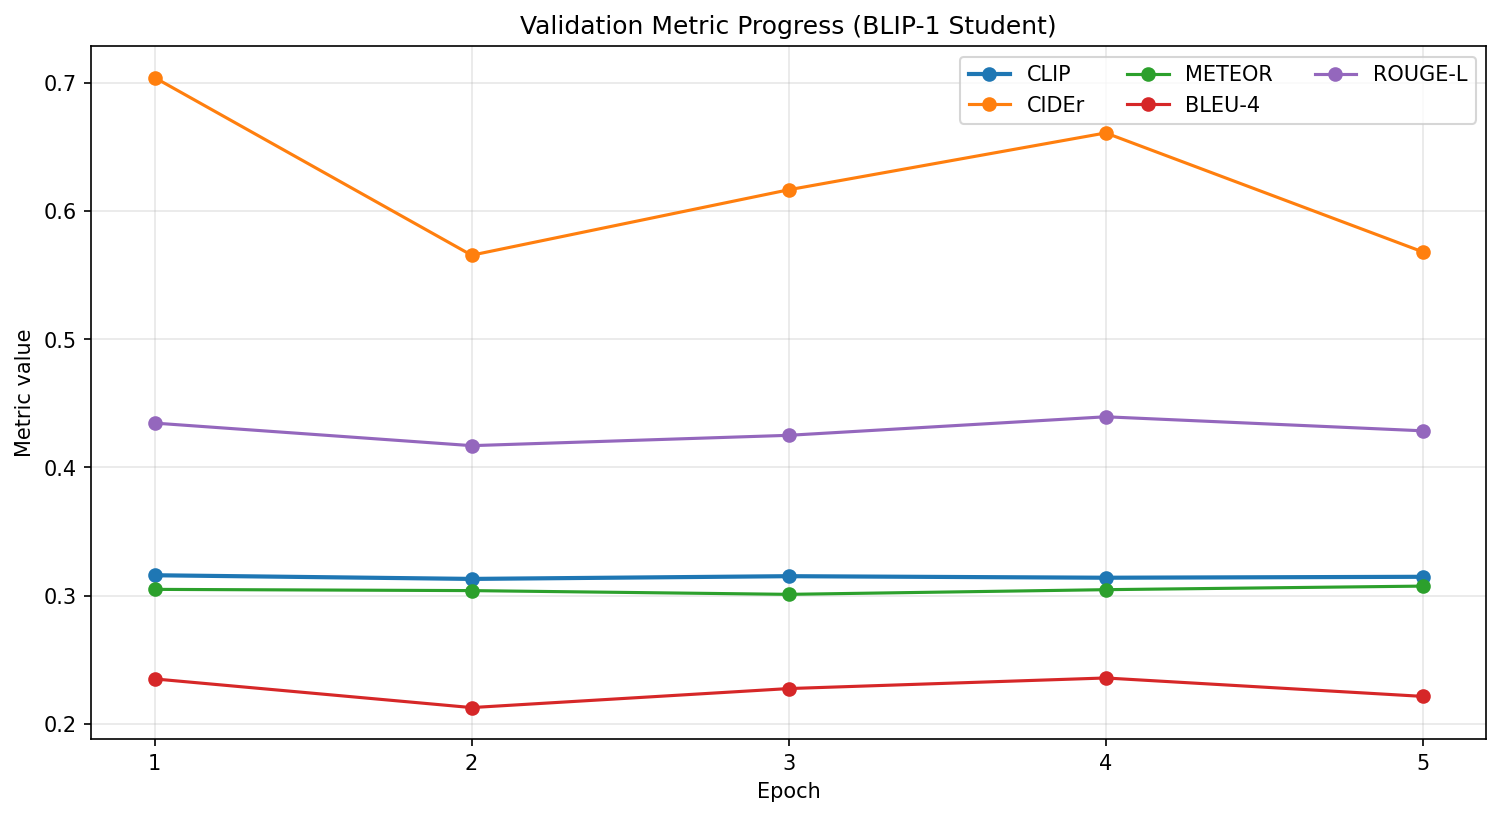
\includegraphics[width=0.9\columnwidth]{graphs/metric_curves_distill.png}}
  \caption{Validation metric progress over 5 epochs. CLIP is stable for both models; METEOR and ROUGE-L improve more steadily in the teacher than the student.}
  \label{fig:metrics_both}
\end{figure}

Fig.~\ref{fig:metrics_both} compares validation metric trajectories. In the teacher, METEOR and ROUGE-L increase steadily through epoch~4 while CIDEr peaks at epoch~4 then drops at epoch~5, motivating composite score checkpoint selection. The student shows a different pattern: CIDEr peaks early and oscillates, while METEOR and ROUGE-L plateau quickly, consistent with the student's reduced capacity.

Fig.~\ref{fig:training_both} shows the corresponding training loss dynamics. The teacher's total loss drops sharply in epoch~1 and stabilizes thereafter, while the student converges more quickly with validation CE remaining stable at $\sim$2.2, reflecting the distillation signal constraining the student's output distribution.

\begin{figure*}[!t]
  \centering
  \subfloat[LoRA teacher. Loss drops sharply in epoch~1 and stabilizes.\label{fig:training}]{%
    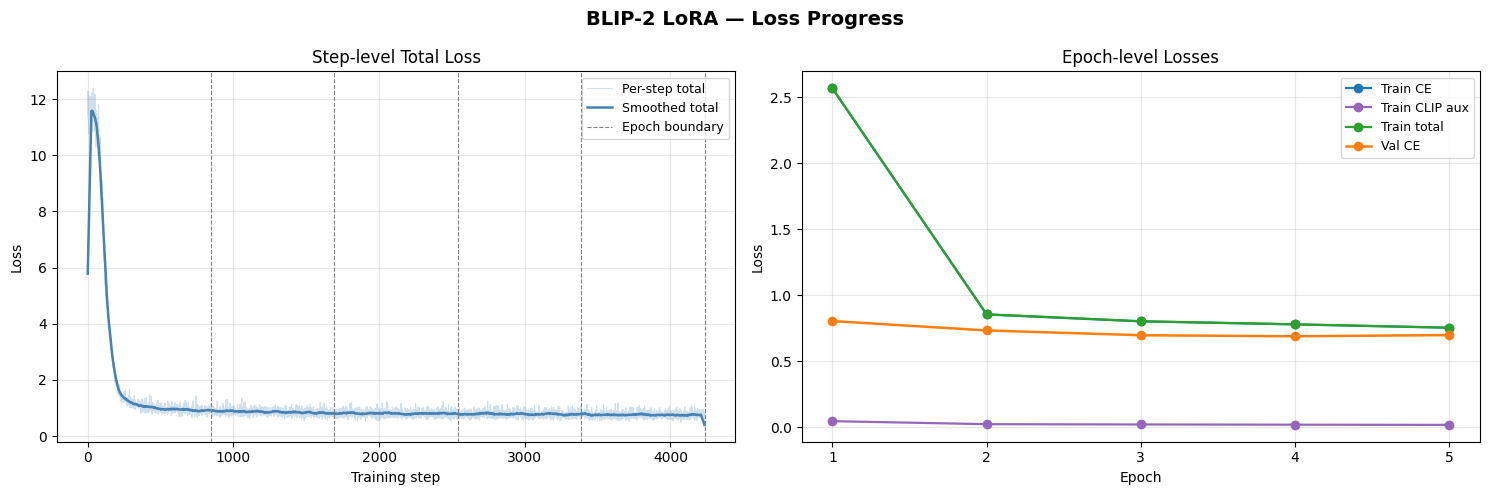
\includegraphics[width=0.82\linewidth]{graphs/loss_curves.png}}\\
  \subfloat[Distilled BLIP-1 student. Loss converges quickly; validation CE stable at $\sim$2.2.\label{fig:training_distill}]{%
    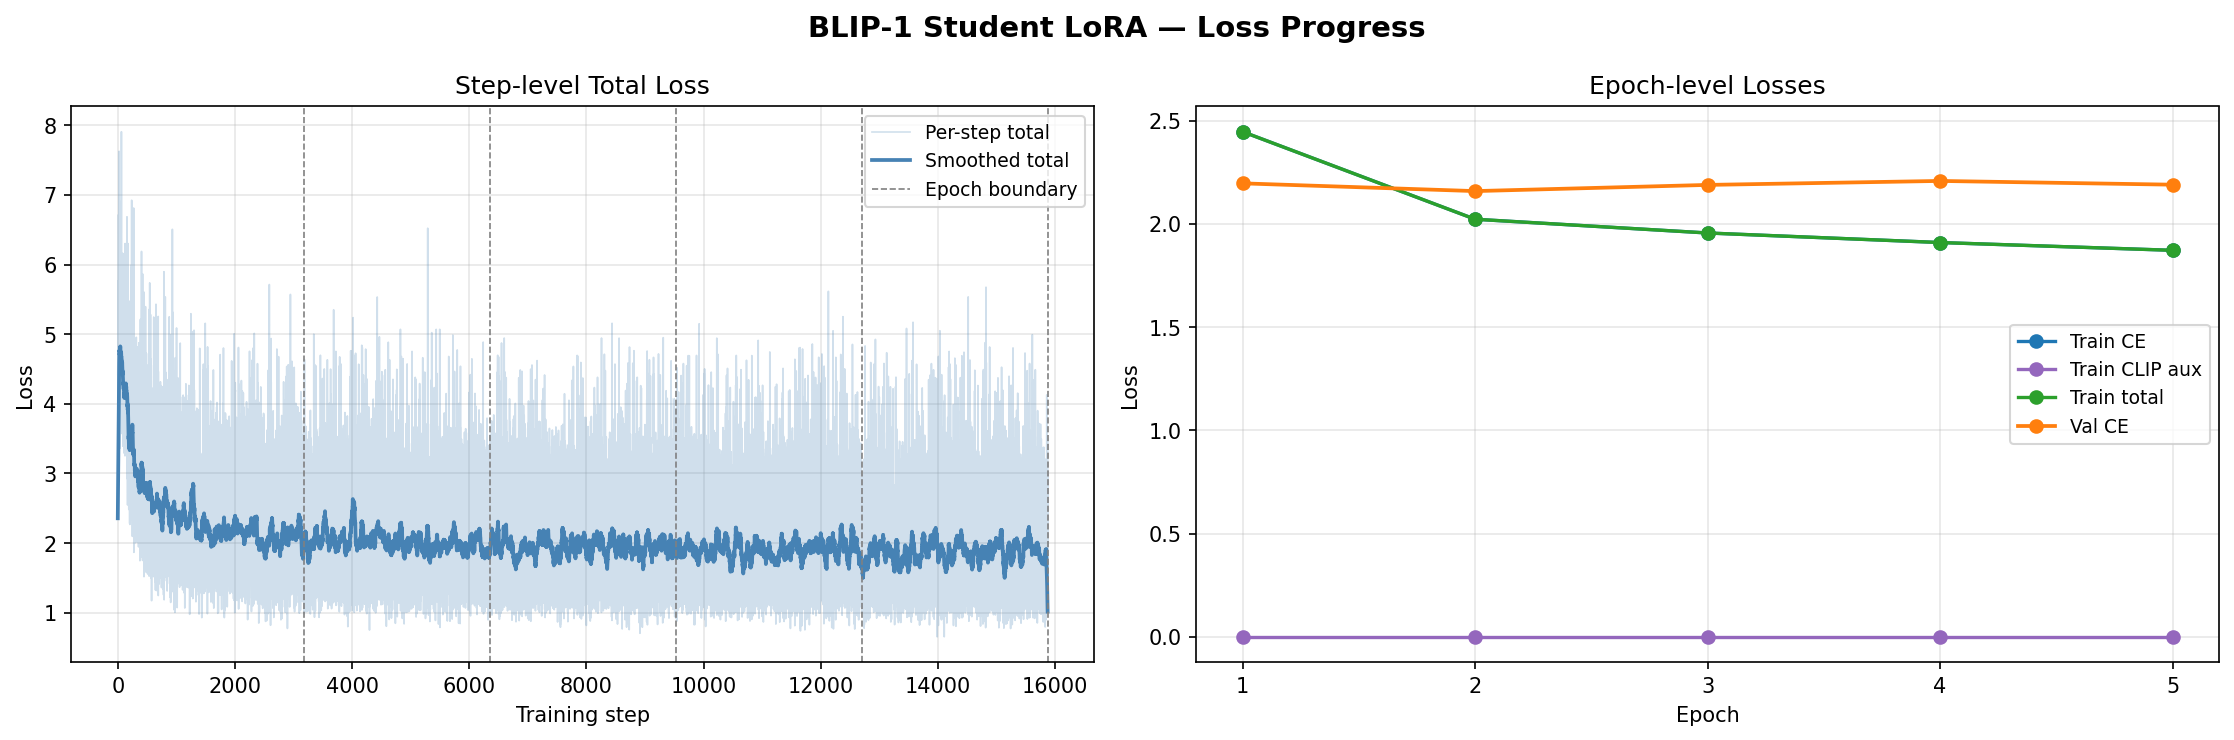
\includegraphics[width=0.82\linewidth]{graphs/loss_curves_distill.png}}
  \caption{Training loss dynamics over 5 epochs. Each panel: per step total loss (left) and epoch level breakdown of train CE, CLIP auxiliary, total, and validation CE (right).}
  \label{fig:training_both}
\end{figure*}

\subsection{Discussion}
The pipeline bridges the domain gap through two complementary mechanisms. The frozen ViT encoder, pretrained on large scale natural image data, yields features that tolerate color shift better than gross structural change: a blue green cast perturbs the histogram but leaves object boundaries, texture, and layout largely intact, so patch based attention still extracts scene level structure in degraded underwater frames. That stability is consistent with the small change in CLIP similarity for the base model (0.311), because the encoder already provides coarse visual semantics before any adaptation. LoRA then specializes the Q-Former cross attention to emphasize cues that matter for marine scenes (e.g., coral texture, fish shape, and open water), which drives domain specific wording without updating the vision backbone. The CLIP auxiliary loss keeps Q-Former states aligned with CLIP's joint embedding so that lexical gains from cross entropy do not come at the cost of visual grounding.

The empirical pattern matches this account: CIDEr, SPICE, and BLEU rise sharply after LoRA, while CLIP moves only slightly, which indicates that the main remaining gap before adaptation was linguistic and relational precision relative to human references, not coarse image text agreement.

The gap between the LoRA teacher and the distilled student in CIDEr (1.32 versus 0.70) follows in part from BLIP-1's smaller capacity, but also from training the student on teacher pseudo labels without access to human references, so some degradation reflects pseudo label bias and distribution shift rather than parameter count alone. Interpretations of teacher versus student quality should treat that regime as a limitation of caption level distillation in general, not only of this implementation.

Additional limitations are as follows. Images with extreme turbidity may still challenge both models when no explicit restoration is applied. UICD contains 3,176 images, so rare taxa and viewpoints are underrepresented and the models may default to frequent species labels when evidence is weak. The period suffix issue, although handled in post processing, suggests that end of sequence behavior is not fully learned and can add decoding cost in latency sensitive deployments. Finally, failures need not have a single origin: pseudo label error, poor visibility, and decoding artifacts can combine, and the student can inherit stacked mistakes that headline metrics underrepresent in the tail of the error distribution. Improving the student may require stronger pseudo label curation or limited use of ground truth captions during training; we leave such extensions to future work.

\FloatBarrier
\section{Conclusion}

We presented BLIP-2 Explorer, a two-stage pipeline for domain adapted underwater image captioning. In the first stage, LoRA fine tuning of BLIP-2 OPT-2.7B on UICD yields CIDEr 1.32 vs.\ 0.47, SPICE 0.27 vs.\ 0.14, and METEOR 0.33 vs.\ 0.18 over the untuned baseline. The key insight is that the frozen ViT encoder already extracts structurally robust features despite underwater color degradation; LoRA's role is to reweight Q-Former attention toward the visual dimensions most diagnostic for marine subjects, and the CLIP auxiliary loss keeps those representations semantically grounded throughout adaptation.

In the second stage, knowledge distillation into a compact BLIP-1 student trained on teacher pseudo labels reduces peak GPU memory by $4\times$ while retaining competitive quality (CIDEr 0.70, METEOR 0.31, ROUGE-L 0.44), enabling practical deployment on embedded marine platforms.

At the system level, the two-stage design separates the teacher, which maximizes caption quality under domain shift, from the student, which targets the memory and latency constraints of embedded marine hardware; this separation simplifies updates when either the base model family or the onboard platform changes.
The same sequence (freeze a strong vision encoder, specialize the language interface with LoRA, then distill) may apply to other niche sensing domains where full finetuning is costly but deployment budgets are tight.
Key contributions include the composite checkpoint selection metric, post processing for period suffix artifacts, and the pseudo label distillation recipe for embedded deployment. Future work will investigate underwater image enhancement as a preprocessing stage, LoRA rank ablations, and qualitative failure analysis across species and depth conditions.

\bibliographystyle{IEEEtran}
\bibliography{references}

\end{document}
